%%%%%%%%%%%%%%%%%%%%%%%%%%%%%%%%%%%%%%%%%%%%%%%%%%%%%%%%%%%%%%%%%%%%%%%%%%%%%%%%
%% BAKALÁRSKA PRÁCA                                                           %%
%%                                                                            %%
%% Názov (sk): Algoritmy detekcie a korekcie lokálnych                        %%
%%             znehodnotení digitálneho audio signálu                         %%
%% Názov (en): Algorithms for Detection and Correction of Local               %%
%%             Degradations in Digital Audio Signals                          %%
%%                                                                            %%
%% Autor: Jakub Kúdela                                                        %%
%% Vedúci: Mgr. Daniel Toropila                                               %%
%%                                                                            %%
%% Akademický rok: 2011/2012                                                  %%
%%%%%%%%%%%%%%%%%%%%%%%%%%%%%%%%%%%%%%%%%%%%%%%%%%%%%%%%%%%%%%%%%%%%%%%%%%%%%%%%

\chapter{Objektívny experiment}
Nasledujúca kapitola popisuje priebeh vlastného objektívneho experimentu s vybranými algoritmami pre detekciu a korekciu lokálnych znehodnotení v digitálnych audio nahrávkach. Jeho cieľom je zhodnotenie efektivity jednotlivých prístupov popísaných v práci. Pri realizácii experimentu nám poslúžila vlastná knižnica DAPNet, ktorá bola predstavená v predchádzajúcej kapitole.

\section{Generovanie vstupných dát}
Súčasťou samotného experimentu je generovanie vstupných dát. Potrebné bolo získať nahrávky bez výskytu lokálnych znehodnotení a tiež nájsť spôsob akým by sme mohli tieto nahrávky poškodiť. Myšlienkou pri generovaní dát bolo, že jedine reverzným prístupom môžeme získať poškodenú nahrávku súčasne s jej odpovedajúcou ideálne čistou variantou. Platí to za predpokladu, že neexistuje dokonalý systém pre čistenie poškodených nahrávok. 

Zdrojom nahrávok vybraných pre experiment sa stal portál \cite{Freesound}, z ktorého bolo stiahnutých a použitých celkom dvanásť audio stôp s rozmanitým charakterom bez porušenia licenčných podmienok. Názov a charakter jednotlivých nahrávok je možné vidieť v tabuľke~\ref{tabulka:nahravky}. Všetky vybrané nahrávky boli prevedené do jednotného formátu (súbor WAV, vzorkové rozlíšenie 16-bit, vzorkovacia frekvencia 44100Hz, mono, dĺžka 2000000 vzoriek, hlasitostná normalizácia 80\%). Každá z vybraných dvanástich stôp bola následne vyfiltrovaná do šiestich rôznych frekvenčných rozpätí aplikáciou ToneBytes Vinyl \cite{Vinyl}. Jednotlivé varianty stôp získané filtráciami majú odpovedať charakteru zvuku vinylového média zo šiestich rôznych časových období. Účelom filtrácií bolo priblížiť sa zvukovej podobe nahrávok, ktoré obsahovali dané lokálne znehodnotenia. 

Aplikácia ToneBytes Vinyl umožnila aj vygenerovanie stôp obsahujúcich len nasimulované analógové lokálne poruchy odpovedajúce vybraným obdobiam. Inak povedané, pre každé zo šiestich časových období, počnúc rokmi štyridsiatymi až po súčasnosť, bolo vyfiltrovaných všetkých dvanásť stôp a bola vygenerovaná stopa obsahujúca len lokálne poruchy. 

Ku každej stope obsahujúcej len analógové poruchy bola vygenerovaná odpovedajúca stopa obsahujúca len digitálne poruchy. Stopa s digitálnou poruchou vznikla zo stopy s analógovými znehodnoteniami tak, že každá poškodená vzorka bola nahradená náhodnou vzorkou procesu Gaussovského bieleho šumu. Tabuľka~\ref{tabulka:filtracie} uvádza názvy vyfiltrvaných nahrávok pre dané časové obdobia a názvy odpovedajúcich stôp, ktoré obsahujú len analógové a digitálne poškodenia.

Stopy pozostávajúce len z lokálnych znehodnotení analógového charakteru majú vďaka aplikácii ToneBytes Vinyl, vzhľadom na nastavené obdobie, rozdielne frekvenčné rozmedzie, intenzitu a hustotu. Vygenerované stopy obsahujúce len digitálne znehodnotenia kopírujú hustotu odpovedajúcich analógových predlôh, zatiaľ čo ich intenzita a frekvenčné rozpätie zostávajú nemenné. 

\begin{table}[!h]
\centering
\caption{Nahrávky objektívneho experimentu}
\begin{tabular}{l l}
\hline
Nahrávka & Charakter\\
\hline
S\_01\_?? & letiskový ruch\\
S\_02\_?? & mužský prednes básne\\
S\_03\_?? & akustické bubny\\
S\_04\_?? & ženská reč\\
S\_05\_?? & londýnsky ruch\\
S\_06\_?? & ženská reportáž\\
S\_07\_?? & biely šum\\
S\_08\_?? & akustický klavír\\
S\_09\_?? & elektrický klavír\\
S\_10\_?? & saxofón\\
S\_11\_?? & ženský spev\\
S\_12\_?? & trumpeta\\
\hline
\end{tabular}
\label{tabulka:nahravky}
\end{table}

\begin{table}[!h]
\centering
\caption{Filtrácie a poškodenia objektívneho experimentu}
\begin{tabular}{l l l l}
\hline
Nahrávka & Obdobie & Analógové & Digitálne\\
\hline
S\_??\_01 & 40. roky & A\_01 & D\_01\\
S\_??\_02 & 50. roky & A\_02 & D\_02\\
S\_??\_03 & 60. roky & A\_03 & D\_03\\
S\_??\_04 & 70. roky & A\_04 & D\_04\\
S\_??\_05 & 80. roky & A\_05 & D\_05\\
S\_??\_06 & 90. roky & A\_06 & D\_06\\
\hline
\end{tabular}
\label{tabulka:filtracie}
\end{table}

\section{Nastavenie parametrov}
Zámerom objektívneho experimentu je vyniesť čo najobecnejšie zhodnotenie efektivity predstavených algoritmov. Tendenciou je zhodnotiť kvalitu korekcie a výpovednú hodnotu excitačných signálov pri výkone jednotlivých metód. Problematiku výberu obecne najefektívnejšej detekčnej brány a detekčného modifikátoru v rámci našej práce vynecháme. Pre účely experimentu bola vybraná spoločná brána so stálými parametrami, rovnako nemenný modifikátor a pre všetky testované algoritmy boli stanovené fixné doporučené nastavenia. Taktiež bol pre rámec experimentu vybraný aj algoritmus pre revízne účely. S jeho úlohou sa oboznámime pri rozbore priebehu experimentu. Podotýkame, že v rámci obecnosti nieje hlavným cieľom experimentu nájdenie najvhodnejších nastavení parametrov vybraných algoritmov pre dané vstupné dáta. Takýmto spôsobom získané najlepšie možné výsledky môžu byť zavádzajúce. Pri niektorých metódach sa totiž vhodné nastavenie parametrov hľadá oveľa komplikovanejšie. Upozorňujeme, že výber spoločnej detekčnej brány a modifikátoru môže do veľkej miery ovplivniť výsledky výskumu. Tie môžu byť rovnako ovplyvnené aj zafixovaním parametrov pre algoritmy vystupujúce v experimente, no v rámci dostupných výpočetných možností bolo potrebné spraviť kompromis. V nasledujúcich zoznamoch máme môžnosť vidieť starostlivo vybranú spoločnú bránu a modifikátor, algoritmus pre revízne účely a nastavenia vybraných algoritmov vystupujúcich v objektívnom experimente. Všetky uvedené nastavenia objektívneho experimentu boli určené na základe doporučenia autorov metód alebo boli vybrané po pozorovaní výsledkov sérií testov. Nastavenia nezachádzajú do extrémov a snažia sa poskytnúť priestor objektivite.

\begin{itemize}
  \item Adaptívna brána smerodajnej odchýlky s dvomi prahmi počítajúca Martin-Kleinerovou approximáciou
  \begin{itemize}
  	\item s parametrami: $P_1=3$, $P_2=2$, $R=20$, $C=50$.
  \end{itemize}
  \item Detekčný prepájač
  \begin{itemize}
    \item s parametrami: $L=1$, $P=25$.
  \end{itemize}
  \item Revízny algoritmus je naivný algoritmus
  \begin{itemize}
      \item s parametrami: $O=5$.
  \end{itemize}
\end{itemize}

\begin{itemize}
  \item Naivný algoritmus 
  \begin{itemize}
    \item s parametrom: $O=5$.
  \end{itemize}
  \item Kasparis-Lanov algoritmus
  \begin{itemize}
    \item s parametrami: $Q=10$, $R=20$, $K=20$.
  \end{itemize}
  \item Autoregresívny algoritmus
  \begin{itemize}
    \item s parametrami: $B=1024$, $P=20$.
  \end{itemize}
  \item Sínusoidovo rozšírený autoregresívny algoritmus
  \begin{itemize}
	\item s parametrami: $B=1024$, $Q=5$, $P=20$.
  \end{itemize}
  \item Algoritmus založený na neurónovej sieti
  \begin{itemize}
    \item s parametrami: $B=512$, $N=20$, $H=5$, $T=100$, $L=0,1$.
  \end{itemize}
\end{itemize}

\section{Priebeh}
Celý objektívny experiment spočíval v monitorovaní výsledkov pre každý z vybraných algoritmov aplikovaný na každú nahrávku poškodenú odpovedajúcimi analógovými a digitálnymi znehodnoteniami v každom časovom období. Proces experimentu zahŕňajúci výpočty s daným algoritmom, nahrávkou a obdobím nazvyme krokom objektívneho experimentu. V jednotlivých krokoch boli zozbierané hodnoty veličín, ktoré si popíšeme pri opise jedného kroku objektívneho experimentu. Na záver si uvedieme z nazbieraných hodnôt výsledné aritmetické priemery a popíšeme si význam takto získaných výsledkov.

Krok objektívneho experimentu pre danú čistú nahrávku v podobe signálu $s$ a signál obsahujúci len lokálne znehodnotenia $g$ prebiehal nasledovne: najskôr bola na signál s poškodeniami $g$ aplikovaná brána s modifikátorom určeným pre experiment, čím sme získali ideálnu detekciu v podobe detekčného signálu $i$. Následne bol znehodnotený čistý signál $s$ signálom poškodení $g$, rešpektujúc charakter poškodení, vo výsledný signál $x$:
$$x_n = \left\{\begin{array}{l l}
	x_n + g_n & \quad \text{$analog$ a $i_n = 1$ (aditívny model)}\\
	g_n & \quad \text{$digital$ a $i_n = 1$ (nahradzujúci model)}\\
	s_n & \quad inak.\\
\end{array} \right.$$
Vzápätí bol prostredníctvom algoritmu získaný excitačný signál $e$ zo znehodnoteného signálu $x$. Opäť bola aplikovaná detekčná brána s modifikátorom, no tentokrát na získaný excitačný signál $e$ vo výsledný analyzovaný detekčný signál $a$. Na poškodený signál $x$ s ideálnym detekčným signálom $i$ bola neskôr aplikovaná korekcia určeného algoritmu, čím sme získali opravený signál $y$. Na rad prišiel revízny algoritmus, ktorý z opraveného signálu získal excitačný, z ktorého sme po ďalšej aplikácií brány a modifikátoru získali revízny detekčný signál $r$.

V rámci jedného kroku objektívneho experimentu boli zozbierané hodnoty nasledovných veličín v snahe popísať kvalitu excitačného signálu určeného algoritmu:
$$D\_Efektivita = \frac{| \{\text{$j$ | $a_j=i_j$} \} |}{| \{\text{$k$ | $i_k=0$ alebo $i_k=1$} \} |} \cdot 100\%,$$
$$N\_Efektivita = \frac{| \{\text{$j$ | $a_j=0$ a $i_j=0$} \} |}{| \{\text{$k$ | $i_k=0$} \} |} \cdot 100\%,$$
$$P\_Efektivita = \frac{| \{\text{$j$ | $a_j=1$ a $i_j=1$} \} |}{| \{\text{$k$ | $i_k=1$} \} |} \cdot 100\%.$$
Veličina $D\_Efektivita$ predstavuje pomer počtu správne označených vzoriek v analyzovanom detekčnom signáli $a$ voči ideálnemu detekčnému signálu $i$ ku počtu vzoriek. Veličina $N\_Efektivita$ reprezentuje pomer počtu správne označených nepoškodených vzoriek v analyzovanej detekcii $a$ voči ideálnej detekcii $i$ ku počtu nepoškodených vzoriek z ideálnej detekcie $i$ a veličina $P\_Efektivita$ je pomer počtu správne označených poškodených vzoriek v analyzovanej detekcii $a$ voči ideálnej detekcii $i$ ku počtu poškodených vzoriek z ideálnej detekcie $i$.

Pre účely sledovania kvality korekcie algoritmu boli v rámci kroku experimentu zaznamenané hodnoty ďalších troch veličín. Prvými dvomi sú priemer absolútnych hodnôt $\bar{d}$ a štandardná odchýlka rozdielov $\sigma_d$ vzoriek čistého signálu $s$ a im odpovedajúcich vzoriek opraveného signálu $y$. Posledná veličina $C\_Efektivita$ je definovaná nasledovne:
$$C\_Efektivita = \frac{| \{\text{$j$ | $r_j=0 $ a $i_j=1$} \} |}{| \{\text{$k$ | $i_k=1$} \} |} \cdot 100\%.$$
Určuje pomer počtu vzoriek, ktoré sú v ideálnej detekcii $i$ označené za poškodené, zatiaľ čo v revíznej detekcii $r$ niesú, ku počtu poškodených vzoriek z ideálnej detekcie $i$. 

V poslednom rade je treba poznamenať, že v rámci krokov objektívneho experimentu boli ešte zaznamenávané časy pre excitáciu a korekciu realizovanú daným algoritmom.


\section{Okenná aplikácia DeclickerInspector}
Vyššie popísaný krok objektívneho experimentu s uvedenými nastaveniami bol implementovaný do Windows Forms aplikácie s názvom DeclickerInspector napísanou v jazyku C\# pod knižnicou DAPNet. Program DeclickerInspector spustíme nasledovným príkazom:\\
\\
\texttt{DeclickerInsecptor.exe (n|kl|ar|sar|nn) (c|d) (samples path) (degradations path) (a|d)}\\
\\
kde \texttt{(n|kl|ar|sar|nn)} je argument reprezentujúci aplikovaný algoritmus (naivný \texttt{n}, Kasparis-Lanov \texttt{kl}, autoregresívny \texttt{ar}, sínusoidovo rozšírený \texttt{sar}, založený na neurónovej sieti \texttt{nn}), argument \texttt{(c|d)} značí vybranú fázu pre ktorú DeclickerInspector zobrazí výsledky (detekčná \texttt{d}, korekčná \texttt{c}), voľba \texttt{(samples path)} je cesta ku súboru s čistým signálom, voľba \texttt{(degradations path)} je cesta ku súboru obsahujúcemu lokálne znehodnotenia a \texttt{(a|d)} je výber modelu pre znehodnotenie signálu (analóg \texttt{a}, digitál \texttt{d}). Všetky z uvedených argumentov sú povinné, rovnako ako je povinné dodržanie ich poradia. 

Po spustení programu pre prehliadanie výsledkov detekcie sa zobrazí okno podobné tomu, ktoré máme možnosť vidieť na obrázku~\ref{obrazok:inspector-detekcia}. Graf nachádzajúci sa v okne zobrazuje stopy znormalizovaného excitačného signálu \textit{Excitations}, čistého signálu \textit{Samples}, stopu signálu lokálnych poškodení \textit{Degradations}, stopu poškodeného vstupného signálu \textit{Degraded} a stopy analyzovanej \textit{Analyzed} a ideálej \textit{Ideal} detekcie. Graf je možné priblížiť a tiež je možné sa v ňom pohybovať prostredníctvom myši. Rozmedzie aktuálne prehliadaného úseku máme možnosť zmeniť aj prostredníctvom textových polí a tlačidiel dostupných v pravom hornom rohu. Štatistiky, nachádzajúce sa v pravom dolnom rohu okna, sú prepočítavané vzhľadom na prehliadaný úsek jednotlivých signálov. Čo sa týka zobrazených štatistík, hodnota veličiny \textit{A\_Number} zobrazuje počet detekovaných sekvencií poškodených vzoriek zvoleným algoritmom v zobrazenom úseku a \textit{A\_Length} udáva priemernú dĺžku týchto sekvencií. Hodnota veličiny \textit{I\_Number} zobrazuje počet detekovaných sekvencií poškodených vzoriek z ideálnej detekcie v zobrazenom úseku, ku ktorým priemerná dĺžka je zobrazená pri veličine \textit{I\_Length}. Polia \textit{D\_Effectivity}, \textit{N\_Effectivity} a \textit{P\_Effectivity} udávajú zaradom hodnoty veličín \textit{D\_Efektivita}, \textit{N\_Efektivita} a \textit{P\_Efektivita} pre prehliadaný úsek.

\begin{figure}[!h]
	\centering
	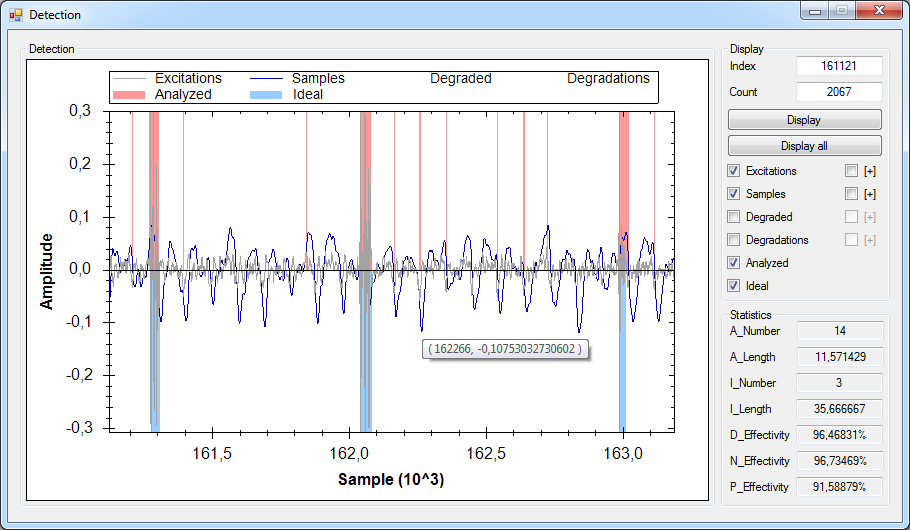
\includegraphics[width=1.0\textwidth]{images/detekcia.png}
	\caption{Aplikácia DeclickerInspector, detekcia}
	\label{obrazok:inspector-detekcia}
\end{figure}

Po spustení aplikácie DeclickerInspector pre korekciu sa zobrazí okno podobné tomu, ktoré je zobrazené na obrázku ~\ref{obrazok:inspector-korekcia}. Rozdiel v okne popisujúcom výsledky korekcie oproti oknu zobrazujúcemu výsledok detekcie je ten, že korekčné okno zobrazuje v grafe namiesto signálu excitácií opravený signál \textit{Corrected} a namiesto analyzovanej detekcie z fázy detekcie zobrazuje revíznu detekciu \textit{Reviewed}. Ďalším rozdielom sú vymenené štatistické veličiny z detekčných za korekčné. Veličiny \textit{Mean} a \textit{Deviation} predstavujú priemer absolútnych hodnôt a štandardnú odchýlku rozdielov vzoriek čistého signálu a odpovedajúcich vzoriek opraveného signálu. Pole \textit{C\_Effectivity} udáva hodnotu veličiny \textit{C\_Efektivita} a význam veličín \textit{I\_Number}, \textit{I\_Length} ostáva rovnaký.

\begin{figure}[!h]
\centering
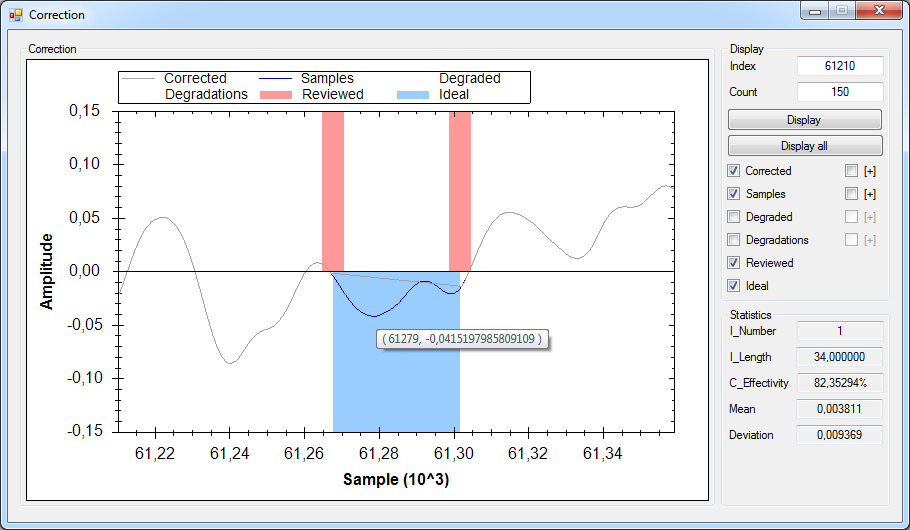
\includegraphics[width=1.0\textwidth]{images/korekcia.png}
\caption{Aplikácia DeclickerInspector, korekcia}
\label{obrazok:inspector-korekcia}
\end{figure}

\section{Výsledky}
V práci bol opísaný priebeh kroku objektívneho experimentu. Ako bolo spomenuté v úvode ku objektívnemu experimentu, pre získanie výsledkov bol zrealizovaný krok pre každý algoritmus so zafixovanými hodnotami parametrov aplikovaný na každú nahrávku v každom časovom období poškodenú odpovedajúcimi analógovými a digitálnymi znehodnoteniami. Nakoniec bol na výsledky aplikovaný aritmetický priemer. V tabuľkách~\ref{tabulka:objektivny-excitacia},~\ref{tabulka:objektivny-korekcia} je možné vidieť úspechy jednotlivých algoritmov (kde N je naivný algoritmus, KL je Kasparis-Laneov, AR je autoregresívny, SAR je sínusoidovo rozšírený autoregresívny a NN je založený na neurónovej sieti).

\begin{table}[!h]
\centering
\caption{Excitačné výsledky objektívneho experimentu}
\begin{tabular}{l l l l l}
\hline
Algoritmus & D\_Efektivita & N\_Efektivita & P\_Efektivita & Čas\\
\hline
N & 87,87 \% & 92,16 \% & 60,64 \% & 36 ms\\
KL & 88,25 \% & 93,74 \% & 59,41 \% & 288 ms\\
AR & 84,87 \% & 88,21 \% & 69,26 \% & 1678 ms\\
SAR & 85,09 \% & 88,63 \% & 68,16 \% & 3474 ms\\
NN & 89,44 \% & 98,00 \% & 28,40 \% & 88025 ms\\
\hline
\end{tabular}
\label{tabulka:objektivny-excitacia}
\end{table}

\begin{table}[!h]
\centering
\caption{Korekčné výsledky objektívneho experimentu}
\begin{tabular}{l l l l l}
\hline
Algoritmus & C\_Efektivita & Priemer & Odchýlka  & Čas\\
\hline
N & 92,26 \% & 0,00759 & 0,02734 & 16 ms\\
KL & 49,09 \% & 0,00768 & 0,02647 & 892 ms\\
AR & 98,79 \% & 0,00400 & 0,01465 & 57016 ms\\
SAR & 98,72 \% & 0,00389 & 0,01425 & 61257 ms\\
NN & 70,00 \% & 0,00738 & 0,02458 & 62450 ms\\
\hline
\end{tabular}
\label{tabulka:objektivny-korekcia}
\end{table}

\section{Zhodnotenie}
Výsledky z excitácií sú uvedené v tabuľke~\ref{tabulka:objektivny-excitacia}. Hodnoty veličiny \textit{D\_Efektivita} reprezentujú množstvo správne označených vzoriek v analyzovanej detekcii voči ideálnej detekcii, kde analyzovaná detekcia vznikne aplikáciou brány a modifikátoru pre objektívny experiment na excitačný sigál. Veličina \textit{N\_Efektivita} značí množstvo správne označených vzoriek v analyzovanej detekcii spomedzi nepoškodených voriek z ideálnej detekcie a hodnota veličiny \textit{P\_Efektivita} symbolizuje množstvo správne označených vzoriek v anazlyzovanej detekcii spomedzi poškodených vzoriek z ideálnej detekcie. Vyššia hodnota veličiny \textit{D\_Efektivita} znamená väčšiu presnosť pri označovaní poškodenosti jednotlivých vzoriek. Vyššia \textit{N\_Efektivita} znamená väčšiu pravdepodobnosť pre označenie nepoškodenej vzorky za nepoškodenú a vyššia \textit{P\_Efektivita} značí väčšiu pravdepodobnosť pre označenie poškodenej vzorky za poškodenú. 

Z tabuliek obsahujúcich výsledky pre excitácie signálu ~\ref{tabulka:objektivny-excitacia}, vyplíva, že hoci je $D\_Efektivita$ veľmi podobná pre všetky vybrané algoritmy (v rozpätí piatich percent), existujú isté kvalitatívne rozdiely v excitačných signáloch. Rozdiely sú evidentné v rámci hodnôt zvyšných dvoch efektivít. Naivný algoritmus má prekvapujúco dobré výsledky. Môže to byť opodstatnené charakterom testovacích dát, pretože všetky lokálne znehodnotenia mali relatívne vysoké frekvenčné zastúpenie. Z výsledkov je ďalej vidno, že Kasparis-Lanov algoritmus je na tom veľmi podobne ako naivný. Rozumné vysvetlenie pre podobnosť výsledkov naivného algoritmu a Kasparis-Lanovho môže podať fakt, že v rámci experimentu bol použitý detekčný modifikátor, ktorý vylepšil výsledky naivného algoritmu natoľko, že sa výsledky týchto dvoch algoritmov priblížili. Od rozšíreného autoregresívneho algoritmu sínusoidovým modelom by sa dali očakávať lepšie výsledky než od nerozšíreného algoritmu, no v tabuľkách môžeme vidieť, že tieto výsledky sú si veľmi podobné. Dôvodom pre podobnosť výsledkov autoregresívneho algoritmu a jeho rozšírenia je charakter vstupných nahrávok. Sínusoidové rozšírenie si kladie za cieľ poskytovať lepšie výsledky pokiaľ ide o nahrávky harmonického charakteru. Množina testovacích dát bola však do značnej miery neharmonická. Na hodnotách jednotlivých efektivít týkajúcich sa excitácie signálu pre vlastný algoritmus založený na neurónovej sieti vidno, že síce je jeho \textit{D\_Efektivita} najlepšia, jeho \textit{P\_Efektivita} však značne zaostáva. Malá \textit{P\_Efektivita} algoritmu značí jeho opatrnosť pri excitácií danej vzorky. V poslednom rade môžeme v tabuľke~\ref{tabulka:objektivny-excitacia} vidieť veličinu, ktorej hodnoty sa zásadne líšia. Je ňou priemerný čas trvania konštrukcie excitačných signálov pri vybraných algoritmoch. Upozorňujeme však, že jednotlivé algoritmy boli implementované uprednostňovaním čistoty kódu pred časovou aj pamäťovou výpočetnou náročnosťou. Napriek tomu nám jednotlivé časy môžu poskytnúť predstavu o empirickej časovej zložitosti uvedených algoritmov. Z výsledkov sa nedá obecne povedať, ktorý z algoritmov obstál pri excitácii signálov najlepšie. Všetko závisí od toho, či je potrebné sa zamerať na správne označovanie poškodených alebo nepoškodených vzoriek. V tabuľke~\ref{tabulka:objektivny-excitacia} vidno, že vybrané algoritmy majú rozdielne priority.

Výsledky z korekcií sú uvedené v tabuľke~\ref{tabulka:objektivny-korekcia}. Hodnoty veličiny \textit{C\_Efektivita} reprezentujú množstvo vzoriek označených za nepoškodené v revíznej detekcii z tých, ktoré boli v ideálnej označené za poškodené. Pre revízne účely objektívneho experimentu bol predom vybraný naivný algoritmus, ktorý dosiahol v experimente so zafixovanými nastaveniami na daných nahrávkach \textit{D\_Efektivitu} vo výške 87,86 \%. Existuje teda určitý predpoklad, že s takouto pravdepodobnosťou taktiež správne určí poškodenosť jednotlivých vzoriek už opraveného signálu. Výška hodnoty \textit{C\_Efektivita} nám v istom slova zmysle určuje mieru zachovanej spojitosti signálu v sekvenciách opravených vzoriek. Ako sme už pri opise priebehu experimentu vysvetlili, $Priemer$ a \textit{Odchýlka} reprezentujú hodnoty priemeru absolútnych hodnôt a štandardných odchýlok rozdielov vzoriek opraveného signálu s im odpovedajúcimi vzorkami pôvodného nepoškodeného signálu. 

Pokiaľ ide o pozorované veličiny, môžeme z tabuľky~\ref{tabulka:objektivny-korekcia} vyčítať, že autoregresívny algoritmus spolu s jeho rozšírením preukázali najžiadanejšie výsledky, naivný algoritmus prekvapil vzhľadom na svoju jednoduchosť, zatiaľ čo Kasparis-Lanov algoritmus by mohol nejedného čitateľa tejto práce sklamať. Vlastný algoritmus založený na neurónových sietiach sa výsledkami nezaradil medzi najlepšie, čo môže byť do značnej miery spôsobené nízkym počtom tréningových iterácií nastavených kvôli obmedzeným výpočetným prostriedkom.

V rámci úplnosti informácie o emprických časových hodnotách si v tabuľke ~\ref{tabulka:pocitac-os} uveďme špecifikáciu inak nezaneprázdneného výpočetného stroja s operačným systémom, na ktorom bol objektívny experiment spustený.

\begin{table}[!h]
\centering
\caption{Systém pre objektívny experiment}
\begin{tabular}{l l}
\hline
Operačný systém & Windows 7 Professional 64-bit\\
Procesor & Intel\textsuperscript{\textregistered} Core\textsuperscript{\texttrademark} i7-2600 CPU @ 3,40 GHz\\
Operačná pamäť & 8 GB\\
\hline
\end{tabular}
\label{tabulka:pocitac-os}
\end{table}